\centering
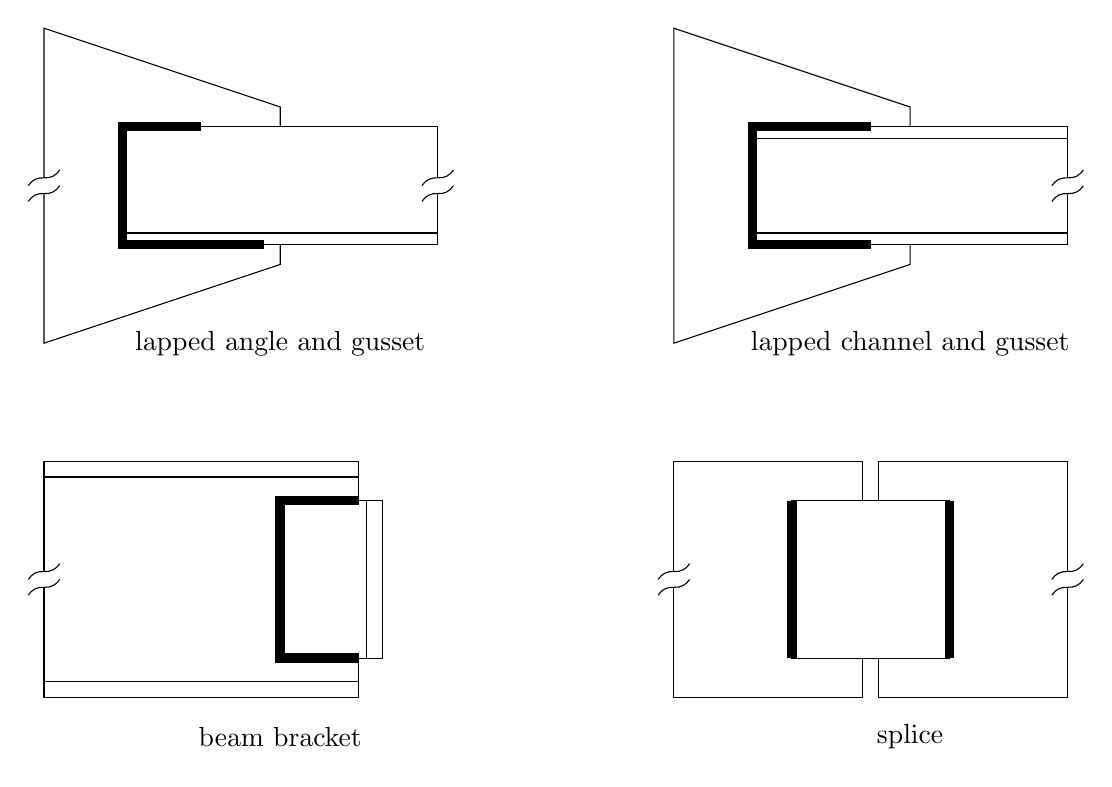
\begin{tikzpicture}[scale=1,ext/.pic={
\path[fill=white](-0.2,0)to[bend left](0,0.1)to[bend right](0.2,0.2)to(0.2,0)to[bend left](0,-0.1)to[bend right](-0.2,-0.2)--cycle;
\draw(-0.2,0)to[bend left](0,0.1)to[bend right](0.2,0.2) (0.2,0)to[bend left](0,-0.1)to[bend right](-0.2,-0.2);
}]
\draw(2,-1)--(2,1)--(-1,2)--(-1,-2)--cycle;
\draw[fill=white](0,-.75)rectangle(4,.75);
\draw(0,-.6)--(4,-.6);
\draw(4,0)pic{ext}(-1,0)pic{ext};
\draw[line width=1.2mm](1,.75)-|(0,-.75)--++(1.8,0);
\node at(2,-2){lapped angle and gusset};
\begin{scope}[xshift=8cm]
\draw(2,-1)--(2,1)--(-1,2)--(-1,-2)--cycle;
\draw[fill=white](0,-.75)rectangle(4,.75);
\draw(0,-.6)--(4,-.6)(0,.6)--(4,.6);
\draw(4,0)pic{ext};(-1,0)pic{ext};
\draw[line width=1.2mm](1.5,.75)-|(0,-.75)--++(1.5,0);
\node at(2,-2){lapped channel and gusset};
\end{scope}
\begin{scope}[yshift=-5cm]
\draw(3,-1.5)rectangle(-1,1.5);
\draw(3,-1.3)--++(-4,0)(3,1.3)--++(-4,0);
\draw[fill=white](2,-1)rectangle(3.3,1);
\draw(3.1,1)--++(0,-2);
\draw(-1,0)pic{ext};
\draw[line width=1.2mm](3,-1)-|(2,1)--++(1,0);
\node at(2,-2){beam bracket};
\begin{scope}[xshift=8cm]
\draw(1.4,-1.5)rectangle(-1,1.5);
\draw(1.6,-1.5)rectangle(4,1.5);
\draw[fill=white](.5,-1)rectangle(2.5,1);
\draw(-1,0)pic{ext}(4,0)pic{ext};
\draw[line width=1.2mm](.5,-1)--++(0,2)(2.5,-1)--++(0,2);
\node at(2,-2){splice};
\end{scope}
\end{scope}
\end{tikzpicture}